\RequirePackage{lineno}
\documentclass[12pt]{article}
\usepackage[utf8]{inputenc}
\usepackage{fullpage}
\usepackage[T1]{fontenc}
\usepackage{amsmath, amsthm, amssymb,amsfonts}
\usepackage{mathptmx}
\usepackage{mathtools}
\usepackage{graphicx}
\usepackage{authblk} % To add authors' affiliations
\usepackage[absolute,overlay]{textpos}
\usepackage{braket}  % bra-ket notation
\usepackage{slashed} % Dirac notation
\usepackage{tikz-feynman,contour}
\usepackage{breqn}   % Equation breaking
% Should I use SIUnitX instead?
\usepackage{units}

\usepackage{hyperref}
\hypersetup{colorlinks,
            citecolor=blue,
            filecolor=black,
            linkcolor=black,
            urlcolor=black
}

\title{Measurement of the neutrino magnetic moment at the NOvA experiment\\ \vspace*{1cm} \texttt{Technical note}}
\author[1]{Robert Kralik}
\affil[1]{University of Sussex, Brighton, UK}
\date{\today}

%\usepackage[printwatermark]{xwatermark}
%\newwatermark[allpages,color=black!20,angle=45,scale=2,xpos=0,ypos=0]{WORK IN PROGRESS}

\usepackage{hyperref}
\hypersetup{
    colorlinks,
    citecolor=blue,
    filecolor=black,
    linkcolor=black,
    urlcolor=black
}

%\linenumbers % Include line numbers

\begin{document}
\maketitle

\begin{abstract}
    This is the abstract
\end{abstract}
\newpage
\tableofcontents
\newpage

\section{Introduction}

Main motivations for the analysis. Briefly mention that there was a previous study by Biao, what were the results there and what limitations (or maybe talk about this in the Experimental overview?).

Maybe briefly mention the overview of the theory and experimental overview.

%The same types of experimental measurements are also sensitive to more exotic neutrino electromagnetic properties: magnetic moments and millicharges, which would be certainly due to new physics beyond the Standard Model. The discovery of millicharges or anomalously large neutrino magnetic moments would have also important implications for astrophysics and cosmology. [NeutrinoPropertiesSnowmass2022.pdf]

%neutrino electromagnetic interactions [...] provide powerful tools to probe the physics beyond the standard model. ... Hence, the theoretical and experimental study of neutrino electromagnetic interactions is a powerful tool in the search for the fundamental theory beyond the standard model. Moreover, the electromagnetic interactions of neutrinos can generate important effects, especially in astrophysical environments, where neutrinos propagate over long distances in magnetic fields in vacuum and in matter. Unfortunately, in spite of many efforts in the search of neutrino electromagnetic interactions, up to now there is no positive experimental indication in favor of their existence. However, it is expected that the standard model neutrino charge radii should be measured in the near future. This will be a test of the standard model and of the physics beyond the standard model which contributes to the neutrino charge radii. Moreover, the existence of neutrino masses and mixing implies that neutrinos have magnetic moments. Since their values depend on the specific theory which extends the standard model in order to accommodate neutrino masses and mixing, experimentalists and theorists are eagerly looking for them. [nuElmagInt2015.pdf]

%The importance of neutrino electromagnetic properties was first mentioned by Pauli in 1930, when he postulated the existence of this particle and discussed the possibility that the neutrino might have a magnetic moment (Pauli, W., 1991, Cambridge Monogr. Part. Phys., Nucl. Phys., Cosmol. 1, 1.). [nuElmagInt2015.pdf]

%Systematic theoretical studies of neutrino electromagnetic properties started after it was shown that in the extended standard model with right-handed neutrinos the magnetic moment of a massive neutrino is, in general, nonvanishing and that its value is determined by the neutrino mass (Lee and Shrock, 1977; Marciano and Sanda, 1977; Petcov, 1977; Fujikawa and Shrock, 1980; Pal and Wolfenstein, 1982; Shrock, 1982; Bilenky and Petcov, 1987). Neutrino electromagnetic properties are important because they are directly connected to fundamentals of particle physics. For example, neutrino electromagnetic properties can be used to distinguish Dirac and Majorana neutrinos, because Dirac neutrinos can have both diagonal and offdiagonal magnetic and electric dipole moments, whereas only the off-diagonal ones are allowed for Majorana neutrinos (Schechter and Valle, 1981; Kayser, 1982, 1984; Nieves, 1982; Pal and Wolfenstein, 1982; Shrock, 1982). Another important case in which Dirac and Majorana neutrinos have quite different observable effects is the spin-flavor precession in an external magnetic field discussed in Sec. VI.B. Neutrino electromagnetic properties are also probes of new physics beyond the standard model, because in the standard model neutrinos can have only a charge radius. The discovery of other neutrino electromagnetic properties would be a signal of new physics beyond the standard model (Bell et al., 2005, 2006; Bell, 2007; Novales-Sanchez et al., 2008). [nuElmagInt2015.pdf]

%Considering an experiment which does not observe any effect of neutrino magnetic moment and obtains a limit on the neutrino mag. moment, it is possible to obtain, following Studenikin (2014), a bound on neutrino millicharge by demanding that the effect of neutrino millicharge is smaller that tha of neutrino magnetic moment. [nuElmagInt2015.pdf - page 580]

\section{Literature review}
\subsection{Theoretical overview}
%Neutrino electromagnetic properties have been proposed since the very beginning by Pauli to solve the discrepancies in the electron beta emission spectra. This was solved by discovering the neutron. Then again, neutrino magnetic moment was proposed as one of the solution to the solar neutrino problem 

\subsection{Electromagnetic properties of the neutrino}

%In the Standard Model (SM) neutrinos are electrically neutral and do not interact with photons at the tree level. However, radiative corrections generate neutrino interactions with photons through loops involving the charged leptons and the W boson, as shown by the one-loop diagrams in Fig. 9(a). The corresponding neutrino-photon interactions are described by charge radii of the flavor neutrinos . Therefore, even in the SM, where neutrinos are neutral and massless, there are non-zero neutrino electromagnetic properties. [NeutrinoPropertiesSnowmass2022.pdf]

% Although in the standard model neutrinos are electrically neutral and do not possess electric or magnetic dipole moments, they have a charge radius which is generated by radiative corrections. [...] In many extensions of the standard model neutrinos also acquire electromagnetic properties through quantum loop effects which allow direct interactions of neutrinos with electromagnetic fields and electromagnetic interactions of neutrinos with charged particles. Hence, the theoretical and experimental study of neutrino electromagnetic interactions is a powerful tool in the search for the fundamental theory beyond the standard model. Moreover, the electromagnetic interactions of neutrinos can generate important effects, especially in astrophysical environments, where neutrinos propagate over long distances in magnetic fields in vacuum and in matter. [nuElmagInt2015.pdf]

% ...the existence of neutrino masses and mixing implies that neutrinos have magnetic moments. Since their values depend on the specific theory which extends the standard model in order to accommodate neutrino masses and mixing, experimentalists and theorists are eagerly looking for them. [nuElmagInt2015.pdf]

In the standard model, neutrino can have electromagnetic interaction only at a higher order of the perturbative expansion of the interaction - from loop diagrams. 
%But this is only the neutrino charge radius, not the neutrino electric or magnetic moment

%Various theories beyond the Standard Model 
In the one photon approximation, the electromagnetic interactions of a neutrino field $\left(\nu_k\left(x\right), k\in\left\lbrace 1,...,N\right\rbrace\right)$, for $N$ neutrino mass states, can be described by the effective interaction Hamiltonian \cite{nuElmagInt2015.pdf}
\begin{equation}
\mathcal{H}^{\left(\nu\right)}_{em}\left(x\right)=\sum^N_{k,j=1}\overline{\nu}_k\left(x\right)\Lambda^{kj}_{\mu}\nu_j\left(x\right)A^{\mu}\left(x\right)
\end{equation}
and the amplitude of neutrino-to-neutrino interaction for \textbf{Dirac} neutrinos shown on fig.\ref{figFeynman} is
\begin{equation}
\braket{\nu_f\left(p_f\right)|j^{\left(\nu\right)}_{\mu}\left(x\right)|\nu_i\left(p_i\right)}=
e^{i\left(p_f-p_i\right)x}\overline{u}_f\left(p_f\right)\Lambda^{fi}_{\mu}\left(p_f,p_i\right)u_i\left(p_i\right),
\end{equation}
where $p_f$ and $p_i$ are the final and initial four momentums respectively and $u/\overline{u}$ are the solutions to the Dirac equation for a free particle. We take into account possible transitions between different mass states $\nu_i$ and $\nu_f$ \cite{nuElmagInt2015.pdf}.

\begin{figure}
\centering
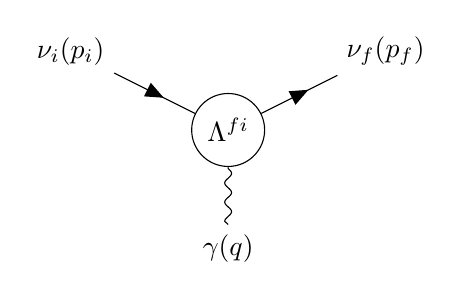
\begin{tikzpicture}
  \begin{feynman}
    \vertex[draw,circle] (m) at ( 0, 0) {$\Lambda^{fi}$};
    \vertex (a) at (-2,1) {\(\nu_i(p_i)\)};
    \vertex (b) at (2,1) {\(\nu_f(p_f)\)};
    \vertex (c) at (0,-1.5) {\(\gamma(q)\)};

    \diagram* {
      (a) -- [fermion] (m) -- [fermion] (b),
      (m) -- [boson] (c)
    };
  \end{feynman}
\end{tikzpicture}
\caption{Effective coupling of neutrinos with one photon electromagnetic field.}
\label{figFeynman}
\end{figure}

The vertex function $\Lambda^{fi}_{\mu}\left(p_f,p_i\right)$ is a matrix and in the most general case it can be written in terms of linearly independent products of Dirac matrices $\left(\gamma\right)$ and four momentum of the photon $\left(q=p_f-p_i\right)$:
\begin{align}
\Lambda^{fi}_{\mu}\left(p_f,p_i\right)=&
\mathbb{F}^{fi}_1\left(q^2\right)q_{\mu}+
\mathbb{F}^{fi}_2\left(q^2\right)q_{\mu}\gamma_5+
\mathbb{F}^{fi}_3\left(q^2\right)\gamma_{\mu}+
\mathbb{F}^{fi}_4\left(q^2\right)\gamma_{\mu}\gamma_5+\notag\\ &
\mathbb{F}^{fi}_5\left(q^2\right)\sigma_{\mu\nu}q^{\nu}+
\mathbb{F}^{fi}_6\left(q^2\right)\epsilon_{\mu\nu\rho\gamma}q^{\nu}\sigma^{\rho\gamma},
\end{align}
where $\mathbb{F}^{fi}_i\left(q^2\right)$ are six Lorentz invariant form factors. For $f=i$ they are called "diagonal" and for $f\neq i$ "transition form factors" \cite{nuElmagInt2015.pdf}.

Applying conditions of hermiticity $\left(\mathcal{H}^{\left(\nu\right)\dagger}_{em}=\mathcal{H}^{\left(\nu\right)}_{em}\right)$ and of conservation of the current (continuity equation: 
$\partial^{\mu}j^{\left(\nu\right)}_{\mu}\left(x\right)=0$), we can rewrite the vertex function as
\begin{equation}
\Lambda^{fi}_{\mu}\left(q\right)=
\left(\gamma_{\mu}-q_{\mu}\slashed{q}/q^2\right)\left[
\mathbb{F}^{fi}_{Q}\left(q^2\right)+\mathbb{F}^{fi}_{A}\left(q^2\right)q^2\gamma_5\right]-
i\sigma_{\mu\nu}q^{\nu}\left[\mathbb{F}^{fi}_{M}\left(q^2\right)+i\mathbb{F}^{fi}_{E}\left(q^2\right)\gamma_5\right],
\end{equation}
where $\mathbb{F}^{fi}_Q,\mathbb{F}^{fi}_M,\mathbb{F}^{fi}_E$ and $\mathbb{F}^{fi}_A$ are hermitian matrices representing the real charge, dipole magnetic, dipole electric and anapole neutrino form factors. In coupling with a real photon $\left(q^2=0\right)$ these become the neutrino charge, magnetic, electric and anapole moment \cite{nuElmagInt2015.pdf}.

For antineutrinos the form factors are transformed as:
\begin{equation}\label{eqAnu1}
\overline{\mathbb{F}}^{fi}_{\Omega}=-\mathbb{F}^{if}_{\Omega}=-\left(\mathbb{F}^{fi}_{\Omega}\right)^{\star} \ \ \ \Omega=Q,M,E,
\end{equation}
\begin{equation}\label{eqAnu2}
\overline{\mathbb{F}}^{fi}_{A}=\mathbb{F}^{if}_{A}=\left(\mathbb{F}^{fi}_{A}\right)^{\star}.
\end{equation}

In case of \textbf{Majorana neutrinos}, the general expression for the vertex function in terms of charge, magnetic, electric and anapole form factors looks the same as for Dirac neutrinos. However, since Majorana antineutrinos are the same particle as Majorana neutrinos, from eq.\ref{eqAnu1},\ref{eqAnu2} we can see that:
\begin{equation}\label{eqAntisymmetryCondition}
\mathbb{F}^M_{\Omega}=-\left(\mathbb{F}^M_{\Omega}\right)^T \ \ \ \Omega=Q,M,E,
\end{equation}
\begin{equation}
\mathbb{F}^M_{A}=\left(\mathbb{F}^M_A\right)^T.
\end{equation}
Therefore the Majorana charge, magnetic and electric form factor matrices are antisymmetric and the anapole form factor matrix is symmetric. This means that Majorana neutrino doesn't have any diagonal charge and dipole magnetic and electric moments, but it can have transition  charge and magnetic and electric moment \cite{nuElmagInt2015.pdf}.

[NuMMBasicsAndAstro\_2022.pdf]
One of the most important for astrophysics consequences of neutrino nonzero effective magnetic moments is the neutrino helicity change $\nu_l\rightarrow\nu_R$ with the appearance of nearly sterile right-handed neutrinos $\nu_R$. In general, this phenomena can proceed in three different mechanisms:
\begin{enumerate}
\item the helicity change in the neutrino magnetic moment scattering on electrons (or protons and neutrons),
\item the neutrino spin and spin-flavour precession in an external magnetic field, and
\item the neutrino spin and spin-flavour precession in the transversally moving matter currents or in the transversally polarized matter at rest
\end{enumerate}
For completeness note that the important astrophysical consequence of nonzero neutrino millicharges is the neutrino deviation from the rectilinear trajectory.

%%%%%%%%%%%%%%%%%%%%%%%%%%%%%%%%%%%%%%%%
\subsubsection{Neutrino electric and magnetic dipole moments}

Evaluating the one loop diagrams in the minimal extension of the standard model with right handed (Dirac) neutrinos gives us the first approximation of the electric and magnetic moments $\left(q^2=0\right)$:
\begin{equation}
\begin{rcases}
\mu^D_{kj}\\
i\epsilon^D_{kj}
\end{rcases}
\simeq\frac{3eG_F}{16\sqrt{2}\pi^2}\left(m_k\pm m_j\right)\left(\delta_{kj}-\frac{1}{2}\sum_{l=e,\mu ,\tau}U^{\star}_{lk}U_{lj}\frac{m_l^2}{m_W^2}\right),
\end{equation}
where $m_k,m_j$ are the neutrino masses, but $m_l$ are the masses of charged leptons which appear in the loop diagrams. Higher order electromagnetic corrections were neglected, but those can also have a significant contribution \cite{nuElmagInt2015.pdf}.

There are no diagonal electric moments $\left(\epsilon_{kk}^D=0\right)$ and the diagonal magnetic moments are approximately
\begin{equation}\label{DiagMagMomVal}
\mu_{kk}^D\simeq\frac{3eG_Fm_k}{8\sqrt{2}\pi^2}\simeq 3.2\times 10^{-19}\left(\frac{m_k}{\textsf{eV}}\right)\mu_B,
\end{equation}
where $\mu_B$ is the Bohr magneton \cite{nuElmagInt2015.pdf}.

The transition magnetic moments are suppressed with respect to the largest of the diagonal magnetic moments by at least a factor of $10^{-4}$ due to the $m_W^2$ in denominator and the transition electric moments are even smaller than that due to the mass difference \cite{nuElmagInt2015.pdf}. Therefore an experimental observation of a magnetic moment larger than in eq.\ref{DiagMagMomVal} would indicate physics beyond the minimally extended standard model \cite{nuMMMajoranaBounds2006.pdf}.

Majorana neutrinos can be obtained by either adding a $\textsf{SU}\left(2\right)_L$ Higgs triplet, or right handed neutrinos together with a $\textsf{SU}\left(2\right)_L$ Higgs singlet. If we neglect the Feynman diagrams which depend on the model of the scalar sector, the magnetic and electric dipole moments are
\begin{equation}
\mu_{kj}^M\simeq -\frac{3ieG_F}{16\sqrt{2}\pi^2}\left(m_k+m_j\right)\sum_{l=e,\mu ,\tau}\operatorname{Im}\left[U^{\star}_{lk}U_{lj}\right]\frac{m_l^2}{m_W^2},
\end{equation}
\begin{equation}
\epsilon_{kj}^M\simeq \frac{3ieG_F}{16\sqrt{2}\pi^2}\left(m_k-m_j\right)\sum_{l=e,\mu ,\tau}\operatorname{Re}\left[U^{\star}_{lk}U_{lj}\right]\frac{m_l^2}{m_W^2}.
\end{equation}
These are difficult to compare to the Dirac case, due to possible presence of Majorana phases in the PMNS matrices, but it is clear that they have the same order of magnitude as Dirac transition dipole moments. However, the neglected model dependent contributions can enhance the transition dipole moments \cite{nuElmagInt2015.pdf}.

It is possible \cite{nuMMMajoranaBounds2006.pdf} to obtain "natural" upper limits on the size of neutrino magnetic moment by calculating its contribution to the neutrino mass by standard model radiative corrections. For Dirac neutrinos the radiative correction induced by neutrino magnetic moment, generated at an energy scale $\Lambda$, to the neutrino mass is generically
\begin{equation}
m_{\nu}^D\sim\frac{\mu_{\nu}^D}{3\times 10^{-15}\mu_B}\left[\Lambda\left(\textsf{TeV}\right)\right]^2\textsf{eV}.
\end{equation}
So for $\Lambda\simeq 1\textsf{TeV}$ and $m_{\nu}\lesssim 0.3\textsf{eV}$ the limit becomes $\mu_{\nu}^D\lesssim 10^{-15}\mu_B$. This applies only if the new physics is well above the electroweak scale ($\Lambda_{EW} \sim 100\textsf{GeV}$). It is possible to get Dirac neutrino magnetic moment higher than this limit, for example in frameworks of minimal super-symmetric standard model, by adding more Higgs doublets, or by considering large extra dimensions \cite{nuElmagInt2015.pdf}.

The limit for Majorana neutrino magnetic moment is less stringent, due to the antisymmetry condition from eq.\ref{eqAntisymmetryCondition} and considering $m_{\nu}\lesssim 0.3\textsf{eV}$ can be expressed as
\begin{align}
\mu_{\tau\mu},\mu_{\tau e} &\lesssim 10^{-9}\left[\Lambda\left(\textsf{TeV}\right)\right]^{-2}\\
\mu_{\mu e} &\lesssim 3\times 10^{-7}\left[\Lambda\left(\textsf{TeV}\right)\right]^{-2}
\end{align}
which is shown in the flavour basis , which relates to the framework used previously as
\begin{equation}
\mu_{ij}=\sum_{\alpha\beta}\mu_{\alpha\beta}U^{\star}_{\alpha i}U_{\beta j},\ \ \ \alpha,\beta\in\left\lbrace e,\mu,\tau\right\rbrace.
\end{equation}
This limits imply, that if a magnetic moment $\mu\gtrsim 10^{-15}\mu_B$ would be measured, it is plausible neutrinos are Majorana fermions and the scale of lepton violation would be well below the conventional see-saw scale \cite{nuMMMajoranaBounds2006.pdf}.

%%%%%%%%%%%%%%%%%%%%%%%%%%%%%%%%%%%%%%%%%%%%%%%%

\subsection{Measuring neutrino magnetic moment}
%Maybe use "Effect of neutrino magnetic moment on measurement" instead
\subsubsection{Effective neutrino magnetic moment}
What we measure in experiments is an effective "flavour" magnetic moment, which is influenced by mixing of "mass" magnetic moments (and electric moments) and oscillations. In the ultrarelativistic limit this is
\begin{equation}
\mu_{\nu_l}^2\left(L,E_{\nu}\right)=\sum_j\left|\sum_k U^{\star}_{lk}e^{-i\Delta m^2_{kj}L/2E_{\nu}}\left(\mu_{jk}-i\epsilon_{jk}\right)\right|^2.
\end{equation}
What is called the effective magnetic moment (often just magnetic moment) therefore contains contributions from both the neutrino magnetic and electric moment \cite{nuElmagInt2015.pdf}.

For antineutrinos, the effective magnetic moment is
\begin{equation}
\mu_{\overline{\nu}_l}^2\left(L,E_{\nu}\right)=\sum_j\left|\sum_k U^{\star}_{lk}e^{+i\Delta m^2_{kj}L/2E_{\nu}}\left(\mu_{jk}-i\epsilon_{jk}\right)\right|^2.
\end{equation}
So the only difference is in the phase induced by neutrino oscillations.

For experiments with baselines short enough for neutrino oscillations to not develop ($\frac{\Delta m^2L}{2E_{\nu}}\ll~1$), such as the NOvA ND, the effective magnetic moment can be expressed as
\begin{equation}
\mu_{\nu_l}^2\simeq\mu_{\overline{\nu}_l}^2\simeq\sum_j\left|\sum_k U_{lk}^{\star}\left(\mu_{jk}-i\epsilon_{jk}\right)\right|^2=\left[U\left(\mu^2+\epsilon^2\right)U^{\dagger}+2\operatorname{Im}\left(U\mu\epsilon U^{\dagger}\right)\right]_{ll^{\prime}},
\end{equation}
which is independent of the neutrino energy and of the source to detector distance.

It is important to mention, that since the effective magnetic moment depends on the flavour of the studied neutrino, it is different for different types of neutrino experiment. Also the solar neutrino experiments need to include the effect of the solar matter on the neutrino oscillations. Therefore the reports on the value (or upper limit) of the effective neutrino magnetic moment are not directly comparable between different types of neutrino experiments.

\subsubsection{Neutrino-on-electron elastic scattering}
The most sensitive method to measure neutrino magnetic moment is the low energy elastic scattering of (anti)neutrinos on electrons \cite{nuElmagInt2015.pdf}. This interaction has two observables, the recoil electron's kinetic energy $\left(T_e\right)$ and the recoil angle with respect to the incoming neutrino beam $\left(\theta\right)$. From simple $2\rightarrow 2$ kinematics we can get
\begin{equation}
\left(P_{\nu}-P_{e^{\prime}}\right)^2=\left(P_{\nu^{\prime}}-P_e\right)^2,
\end{equation}
\begin{equation}
m_{\nu}^2+m_e^2-2E_{\nu}E_{e^{\prime}}+2E_{\nu}p_{e^{\prime}}\cos\theta=m_{\nu}^2+m_e^2-2E_{\nu^{\prime}}m_e.
\end{equation}
Using the energy conservation
\begin{equation}
E_{\nu}+m_e=E_{\nu^{\prime}}+E_{e^{\prime}}=E_{\nu^{\prime}}+T_e+m_e\Rightarrow E_{\nu^{\prime}}=E_{\nu}-T_e
\end{equation}
we get
\begin{equation}
E_{\nu}p_{e^{\prime}}\cos\theta=E_{\nu}E_{e^{\prime}}-E_{\nu^{\prime}}m_e=E_{\nu}\left(T_e+m_e\right)-\left(E_{\nu}-T_e\right)m_e=T_e\left(E_{\nu}+m_e\right),
\end{equation}
\begin{equation}
\cos\theta=\frac{E_{\nu}+m_e}{E_{\nu}}\sqrt{\frac{T_e^2}{E_{e^{\prime}}^2-m_e^2}}=\frac{E_{\nu}+m_e}{E_{\nu}}\sqrt{\frac{T_e^2}{T_e^2+2T_em_e}}.
\end{equation}
And finally we get
\begin{equation}\label{eqThetaTRelation}
\cos\theta=\frac{E_{\nu}+m_e}{E_{\nu}}\sqrt{\frac{T_e}{T_e+2m_e}}.
\end{equation}
Electron's kinetic energy is kinematically constrained by
\begin{equation}
T_e\leq\frac{2E_{\nu}^2}{2E_{\nu}+m_e}.
\end{equation}

Considering $E_{\nu}\sim\textsf{GeV}$, we can approximate $\frac{m_e^2}{E_{\nu}^2}\rightarrow 0$ and in the small angle approximation we get from eq.\ref{eqThetaTRelation} 
\begin{equation}\label{eqTThetaSqExp}
T\theta^2\cong 2m_e\left(1-\frac{T_e}{E_{\nu}}\right)<2m_e.
\end{equation}

In the ultrarelativistic limit, the neutrino magnetic moment changes the neutrino helicity, turning active neutrinos into sterile. Since the SM weak interaction conserves helicity we can add the two contribution to the neutrino on electron cross section incoherently \cite{nuElmagInt2015.pdf}:
\begin{equation}
\frac{d\sigma_{\nu_le^-}}{dT_e}=\left(\frac{d\sigma_{\nu_le^-}}{dT_e}\right)_{\textsf{SM}}+\left(\frac{d\sigma_{\nu_le^-}}{dT_e}\right)_{\textsf{MAG}}.
\end{equation}

The standard model contribution can be expressed as \cite{nuElmagInt2015.pdf}:
\begin{equation}
\left(\frac{d\sigma_{\nu_le^-}}{dT_e}\right)_{\textsf{SM}}=\frac{G_F^2m_e}{2\pi}\left\lbrace\left(g_V^{\nu_l}+g_A^{\nu_l}\right)^2+\left(g_V^{\nu_l}-g_A^{\nu_l}\right)^2\left(1-\frac{T_e}{E_{\nu}}\right)^2+\left(\left(g_A^{\nu_l}\right)^2-\left(g_V^{\nu_l}\right)^2\right)\frac{m_eT_e}{E_{\nu}^2}\right\rbrace,
\end{equation}
where the coupling constants $g_V$ and $g_A$ are different for different neutrino flavours and for antineutrinos. Their values are:
\begin{align}
g_V^{\nu_e}&=2\sin^2\theta_W+1/2,\hspace{2.5cm} g_A^{\nu_e}=1/2,\\
g_V^{\nu_{\mu,\tau}}&=2\sin^2\theta_W-1/2,\hspace{2.25cm} g_A^{\nu_{\mu,\tau}}=-1/2.
\end{align}
For antineutrinos $g_A\rightarrow -g_A$.

Using expressions \ref{eqThetaTRelation} and \ref{eqTThetaSqExp} we can also derive \cite{NuOnECrossSections1989.pdf} cross sections with respect to $\cos\theta$, $\theta^2$ and $T\theta^2$:

\begin{multline}
\left(\frac{d\sigma_{\nu_le^-}}{d\cos\theta}\right)_{\textsf{SM}}=
\frac{2G_F^2E_{\nu}^2m_e^2\cos\theta\left(E_{\nu}+m_e\right)^2}{\pi\left(\left(E_{\nu}+m_e\right)^2-E_{\nu}^2\cos^2\theta\right)^2}\\
\left\lbrace\left(g_V^{\nu_l}+g_A^{\nu_l}\right)^2 +
\left(g_V^{\nu_l}-g_A^{\nu_l}\right)^2\left(1-\frac{2m_eE_{\nu}\cos^2\theta}{\left(E_{\nu}+m_e\right)^2-E_{\nu}^2\cos^2\theta}\right)^2\right. +\\
\left.\left(\left(g_A^{\nu_l}\right)^2-\left(g_V^{\nu_l}\right)^2\right)
\frac{2m_e^2\cos^2\theta}{\left(\left(E_{\nu}+m_e\right)^2-E_{\nu}^2\cos^2\theta\right)}\right\rbrace,
\end{multline}
 
\begin{multline}
\left(\frac{d\sigma_{\nu_le^-}}{d\theta^2}\right)_{\textsf{SM}}=
\frac{G_F^2m_e^2}{\pi\left(\theta^2+\frac{2m_e}{E_{\nu}}\right)^2}
\left\lbrace
\left(g_V^{\nu_l}+g_A^{\nu_l}\right)^2+\left(g_V^{\nu_l}-g_A^{\nu_l}\right)^2
\left(\frac{\theta^2}{\theta^2+\frac{2m_e}{e_{\nu}}}\right)^2\right. +\\
\left.\left(\left(g_A^{\nu_l}\right)^2-\left(g_V^{\nu_l}\right)^2\right)
\frac{2m_e^2}{E_{\nu}^2\left(\theta^2+\frac{2m_e}{E_{\nu}}\right)}\right\rbrace,
\end{multline}

\begin{multline}
\left(\frac{d\sigma_{\nu_le^-}}{dT\theta^2}\right)_{\textsf{SM}}=
\frac{G_F^2E_{\nu}}{4\pi}
\left\lbrace
\left(g_V^{\nu_l}+g_A^{\nu_l}\right)^2+\left(g_V^{\nu_l}-g_A^{\nu_l}\right)^2
\left(\frac{T\theta^2}{2m_e}\right)^2\right. +\\
\left.\left(\left(g_A^{\nu_l}\right)^2-\left(g_V^{\nu_l}\right)^2\right)
\frac{m_e}{E_{\nu}}\left(1-\frac{T\theta^2}{2m_e}\right)\right\rbrace.
\end{multline}

The neutrino magnetic moment contribution is (include derivation from \cite{NeutrinoElmagFormFactors1989.pdf}) \cite{nuElmagInt2015.pdf}:
\begin{equation}
\left(\frac{d\sigma_{\nu_le^-}}{dT_e}\right)_{\textsf{MAG}}=\frac{\pi\alpha^2}{m_e^2}\left(\frac{1}{T_e}-\frac{1}{E_{\nu}}\right)\left(\frac{\mu_{\nu_l}}{\mu_B}\right)^2,
\end{equation}
where $\alpha$ is the fine structure constant.

Analogically to previous, we can also express this cross section in $\cos\theta$, $\theta^2$ and $T\theta^2$:
\begin{equation}
\left(\frac{d\sigma_{\nu_le^-}}{d\cos\theta}\right)_{\textsf{MAG}}=
\frac{2\pi\alpha^2\left(E_{\nu}+m_e\right)^2}{m_e^2\cos\theta}
\frac{\left(E_{\nu}+m_e\right)^2-E_{\nu}^2\cos^2\theta-2m_eE_{\nu}\cos^2\theta}{\left(\left(E_{\nu}+m_e\right)^2-E_{\nu}^2\cos^2\theta\right)^2}
\left(\frac{\mu_{\nu_l}}{\mu_B}\right)^2,
\end{equation}

\begin{equation}
\left(\frac{d\sigma_{\nu_le^-}}{d\theta^2}\right)_{\textsf{MAG}}=\frac{\pi\alpha^2}{m_e^2}\frac{\theta^2}{\left(\theta^2+\frac{2m_e}{E_{\nu}}\right)}\left(\frac{\mu_{\nu_l}}{\mu_B}\right)^2,
\end{equation}

\begin{equation}
\left(\frac{d\sigma_{\nu_le^-}}{dT\theta^2}\right)_{\textsf{MAG}}=\frac{\pi\alpha^2}{4m_e^4}\frac{T\theta^2}{\left(1-\frac{T\theta^2}{2m_e}\right)}\left(\frac{\mu_{\nu_l}}{\mu_B}\right)^2.
\end{equation}

The magnetic moment contribution exceeds the standard model contribution for low enough $T_e$ \cite{nuElmagInt2015.pdf}:
\begin{equation}
T_e\lesssim\frac{\pi^2\alpha^2}{G_F^2m_e^3}\left(\frac{\mu_{\nu}}{\mu_B}\right)^2\simeq 2.9\times 10^{19}\left(\frac{\mu_{\nu}}{\mu_B}\right)^2\left[\textsf{MeV}\right],
\end{equation}
which does not depend on the neutrino energy and makes neutrino experiment sensitive to lower energetic neutrinos more sensitive to the neutrino magnetic moment.
\subsection{Experimental overview}
\RequirePackage{lineno}
\documentclass[12pt]{article}
\usepackage[utf8]{inputenc}
\usepackage{fullpage}
\usepackage[T1]{fontenc}
\usepackage{amsmath, amsthm, amssymb,amsfonts}
\usepackage{mathptmx}
\usepackage{graphicx}

\usepackage{hyperref}
\hypersetup{colorlinks,
            citecolor=blue,
            filecolor=black,
            linkcolor=black,
            urlcolor=black
}

\title{Experimental overview of neutrino magnetic moment measurements}
\date{\today}

%\linenumbers % Include line numbers

\begin{document}
\maketitle

\section{Direct muon (anti)neutrino magnetic moment measurements}
\subsection{NOvA (Biao's thesis)}
\begin{itemize}
    \item $\nu_\mu$ only
    \item Only comparing total event counts - 25 events observed and 23.78 expected
    \item Put an upper limit ($90\%$ C.L.) of $\mu_{\nu_\mu}<1.58\times 10^{-9}\mu_B$ with $10.9\%$ systematic uncertainty on the standard model background
    \item Used $3.62\times 10^{20}$ POT of data ($6.74\times 10^{23}$ POT for MC) with $T\theta^2<0.003\textsf{GeV}\times\textsf{Rad}^2$, $0.3<T<0.9\textsf{GeV}$
\end{itemize}

\subsection{MiniBooNE}
\begin{itemize}
    \item $\nu_\mu$ only
    \item Observed excess of events (seems a bit too high)
\end{itemize}

\subsection{E734 at the Alternating Gradient Synchrotron (AGS) of the Brookhaven National Laboratory}
\begin{itemize}
    \item \textbf{Both $\nu_\mu$ and $\overline{\nu}_\mu$}
    \item $\mu_{\nu_\mu}<8.5\times 10^{-10}\mu_B$
%    \item \href{https://journals.aps.org/prd/abstract/10.1103/PhysRevD.41.3297}
\end{itemize}

\subsection{LSND}

\section{Direct electron (anti)neutrino magnetic moment measurements}

\section{Solar neutrino magnetic moment measurements}
\subsection{XENONnT}
First results published in arXiv:2207.11330\cite{XENON:2022mpc} on 22 July 2022.
\begin{itemize}
    \item 5.9 tonne dual-phase liquid xenon TPC dark matter detector
    \item Region Of Interest is (1,140)~keV
    \item Very low background (~5 times lower than XENON1T)
    \item Tritium excluded as the potential background (also in XENON1T)
    \item No excess found - XENON1T excess excluded with ~4$\sigma$
    \item The $90\%$ C.L. upper limit on solar neutrinos with an "enhanced" magnetic moment is \\$\mu_{\nu_{sol}}~<~6.3\times~10^{-12}\mu_B$, the strongest non-astronomical limit so far (see fig.\ref{fig:XENONnTResults})
\end{itemize}

\begin{figure}
    \centering
    \hspace*{1.5cm}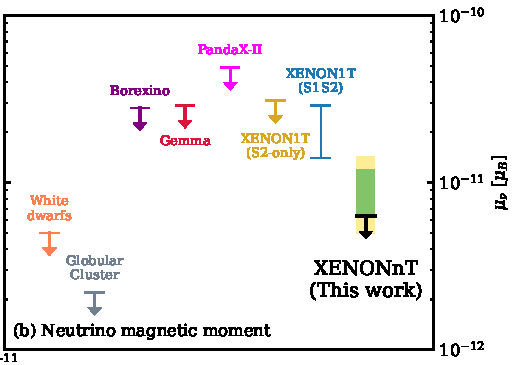
\includegraphics[width=.7\textwidth]{XENONnTExpResultsComparison.pdf}
    \caption{90\% C.L. upper limit on solar neutrinos with an enhanced magnetic moment.}
    \label{fig:XENONnTResults}
\end{figure}
Amir Khan used\cite{Khan:2022bel} XENONnT's results and derived limits on electromagnetic properties for the three SM neutrino flavours (see fig.\ref{fig:XENONnTFit_Khan}).
\begin{figure}
    \centering
    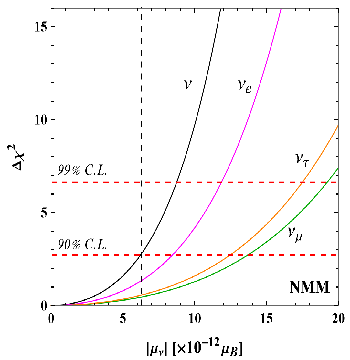
\includegraphics[width=.65\textwidth]{XENONnTFitForNuMM_Khan.pdf}
    \caption{One-dimensional $\Delta\chi^2$ distribution with 90\% and 99\% C.L. boundaries of neutrino magnetic moments. The distribution in black corresponds to the effective flavor independent magnetic moment}
    \label{fig:XENONnTFit_Khan}
\end{figure}
For $\nu_\mu$ they 

\subsection{XENON1T}

\subsection{BOREXINO}

\section{Other}
\subsection{LHC Forward Physics Facilities}
Preliminary sensitivity studies for future experiments (namely for FLArE and FASER$\nu$2)
\begin{itemize}
    \item LHC’s Forward Physics Facilities study high energy (TeV) neutrinos of all flavours from the ATLAS interaction point.
    \item Large opportunity to study tau neutrinos in more detail
\end{itemize}

\bibliographystyle{unsrturl}
\bibliography{ExperimentalOverviewNuMMLiterature}
\end{document}


%%%%%%%%%%%%%%%%%%%%%%%%%%%%%%%%%%%%%%%%%%%%%%%%%%%%%%%%%%%%%%%%%%%%%
%%%                       ANALYSIS OVERVIEW                       %%%
%%%%%%%%%%%%%%%%%%%%%%%%%%%%%%%%%%%%%%%%%%%%%%%%%%%%%%%%%%%%%%%%%%%%%
\section{Analysis overview}
\subsection{Datasets and Event Reconstruction details}
\subsubsection{Enhanced $\nu$-on-e sample}
\subsubsection{Enhance $\nu_e$CC MEC sample}
\subsection{Analysis weights}
\subsubsection{Neutrino magnetic moment as a weight}
\subsubsection{Radiative correction weight}
\subsection{Event selection}
\begin{enumerate}
\item Very brief description of common-sense preselection cuts in decafs
\item Description of all variables used for selection in this analysis
\item Plots of all variables used for selection in this analysis, showing the distribution with L: no cuts and R: cumulative cuts up to this point.
\item Test explaining the motivation for each selection cut.
\end{enumerate}
Describe/point to the ND group's event selection
Plots of event selection variables distribution with two columns. Left distribution with no cuts applied and right with all previous cuts applied.

\subsection{Resolution and binning}
\subsubsection{Fitting framework}

%%%%%%%%%%%%%%%%%%%%%%%%%%%%%%%%%%%%%%%%%%%%%%%%%%%%%%%%%%%%%%%%%%%%%
%%%                   SYSTEMATIC UNCERTAINTIES                    %%%
%%%%%%%%%%%%%%%%%%%%%%%%%%%%%%%%%%%%%%%%%%%%%%%%%%%%%%%%%%%%%%%%%%%%%
\section{Systematic uncertainties}
Plots showing combined uncertainties for signal and backgrounds

\subsection{Normalization systematics}
Should we include normalization systematics?

\subsection{Neutrino flux systematics}
Using the PCA vs using the PPFX universes+beam transport separately. Plots of energy showing shifts for signal and backgrounds separately

[to do]: understand differences with ND and 3F methods

\subsection{Detector systematics}
Plots of energy showing shifts for signal and backgrounds separately
\subsection{Cross section systematics}
Only for the non nu-on-e background. Assuming the nu-on-e events (including the signal events) are precisely known.

Plots of energy showing shifts for signal and backgrounds separately

%%%%%%%%%%%%%%%%%%%%%%%%%%%%%%%%%%%%%%%%%%%%%%%%%%%%%%%%%%%%%%%%%%%%%
%%%                           RESULTS                             %%%
%%%%%%%%%%%%%%%%%%%%%%%%%%%%%%%%%%%%%%%%%%%%%%%%%%%%%%%%%%%%%%%%%%%%%
\section{Results}
[to do]: talk about the shape-only versus normalisation-only strategies for the differential versus single-bin analyses.

\subsection{Counting experiment}
Single bin analysis - total numbers of signal and backgrounds
\subsection{Binned experiment}
Plots showing delta chi2 for stats and systs separately. Plot showing the chi2 with limits
\subsubsection{Sensitivities and limits}

\section{Conclusion}
Report the limit with its uncertainty.

Very briefly discuss differences with current world limit and how the techniques differ.

Very briefly summarise expectations for future measurements.

\bibliographystyle{unsrturl}
\bibliography{NeutrinoMagMomentTechnoteLiterature}
\end{document}
